\documentclass[AutoFakeBold]{LZUThesis}

\usepackage{graphicx}
\usepackage{subfloat} 
\usepackage{diagbox}
\graphicspath{{figures/},{pics/},{images/}} 

\begin{document}


\begin{figure}[htbp]
    \centering
    \subfloat[原始图像]{
        \begin{minipage}[t]{1.0\linewidth}
            \centering
            \includegraphics[width=5cm]{mask_image.jpg}
            \includegraphics[width=5cm]{mask_image1.jpg}
            \includegraphics[width=5cm]{mask_image2.jpg}
            %\caption{fig1}
        \end{minipage}%
    }%
    \quad
    \subfloat[真实分割图]{
        \begin{minipage}[t]{1.0\linewidth}
            \centering
            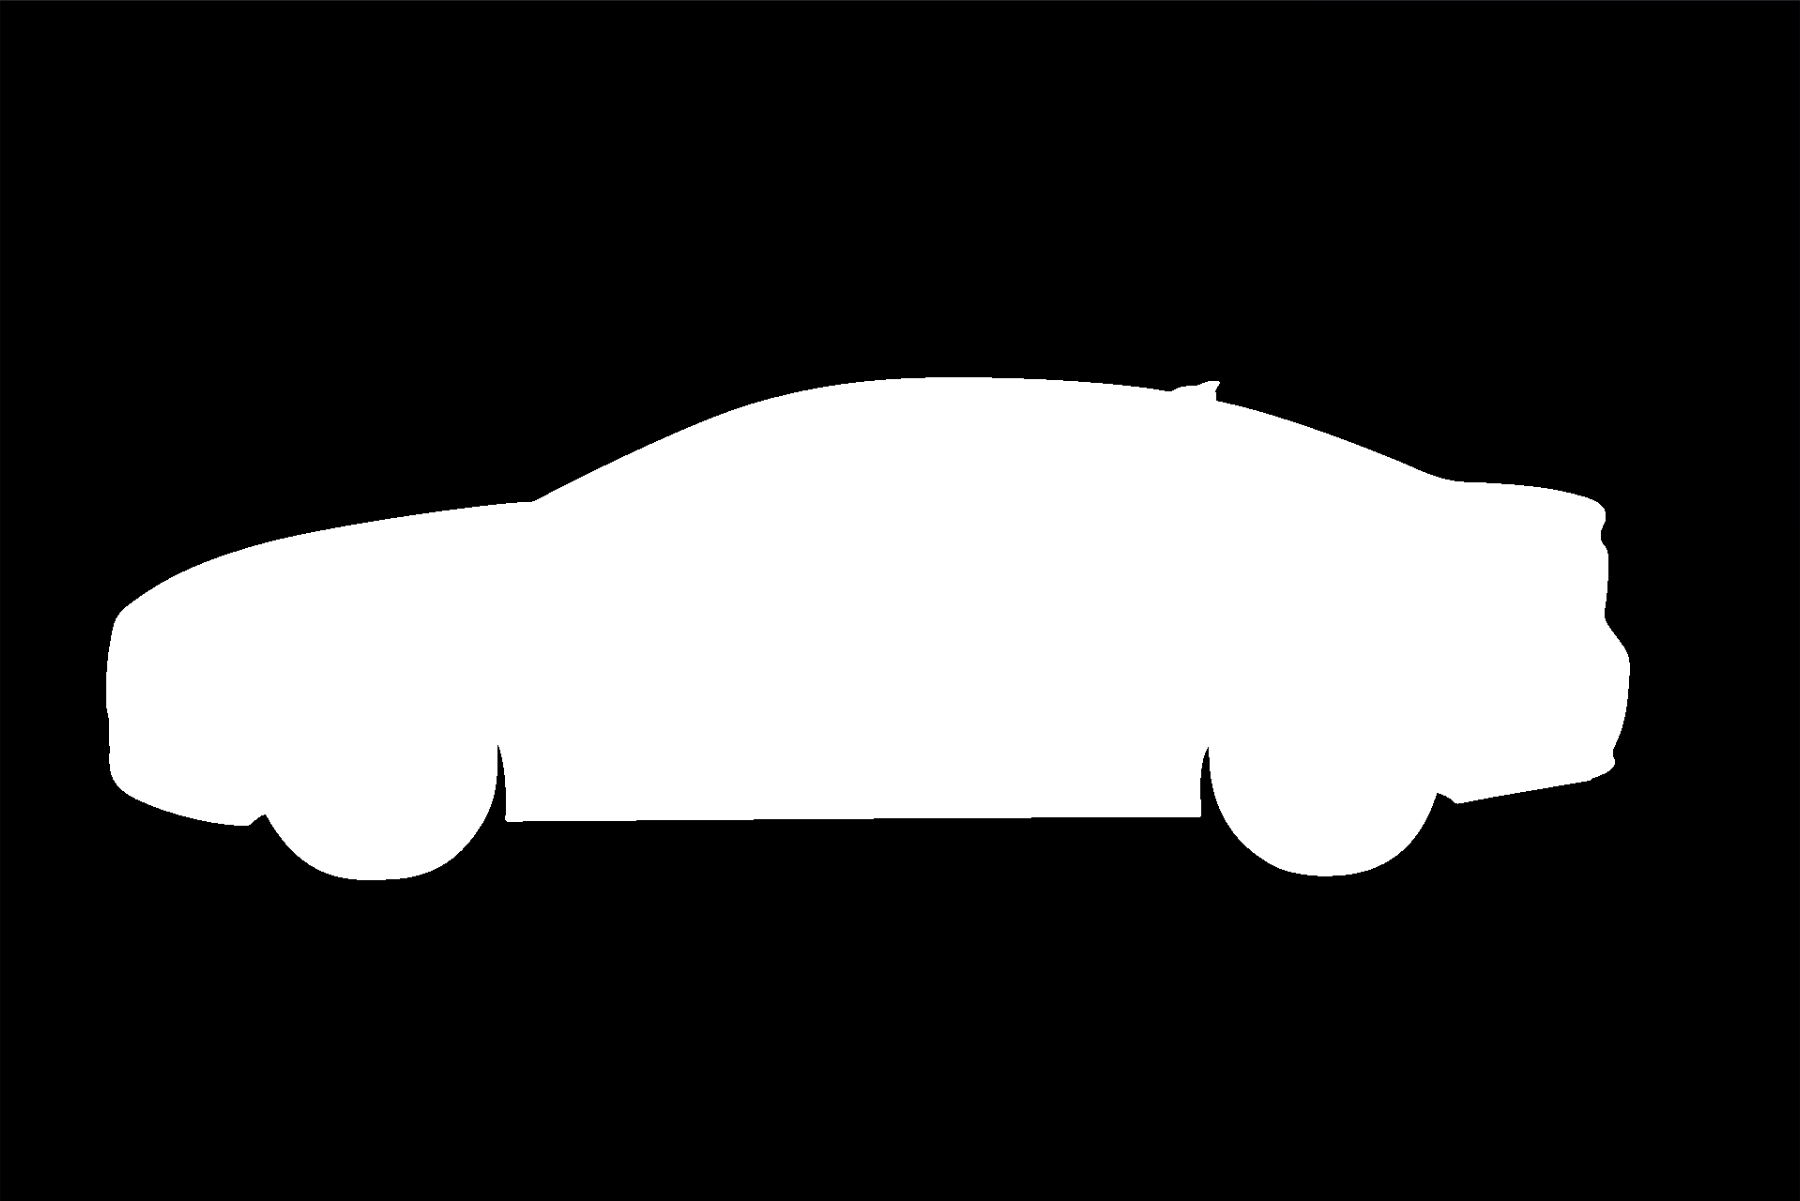
\includegraphics[width=4.5cm]{mask_true.png}
            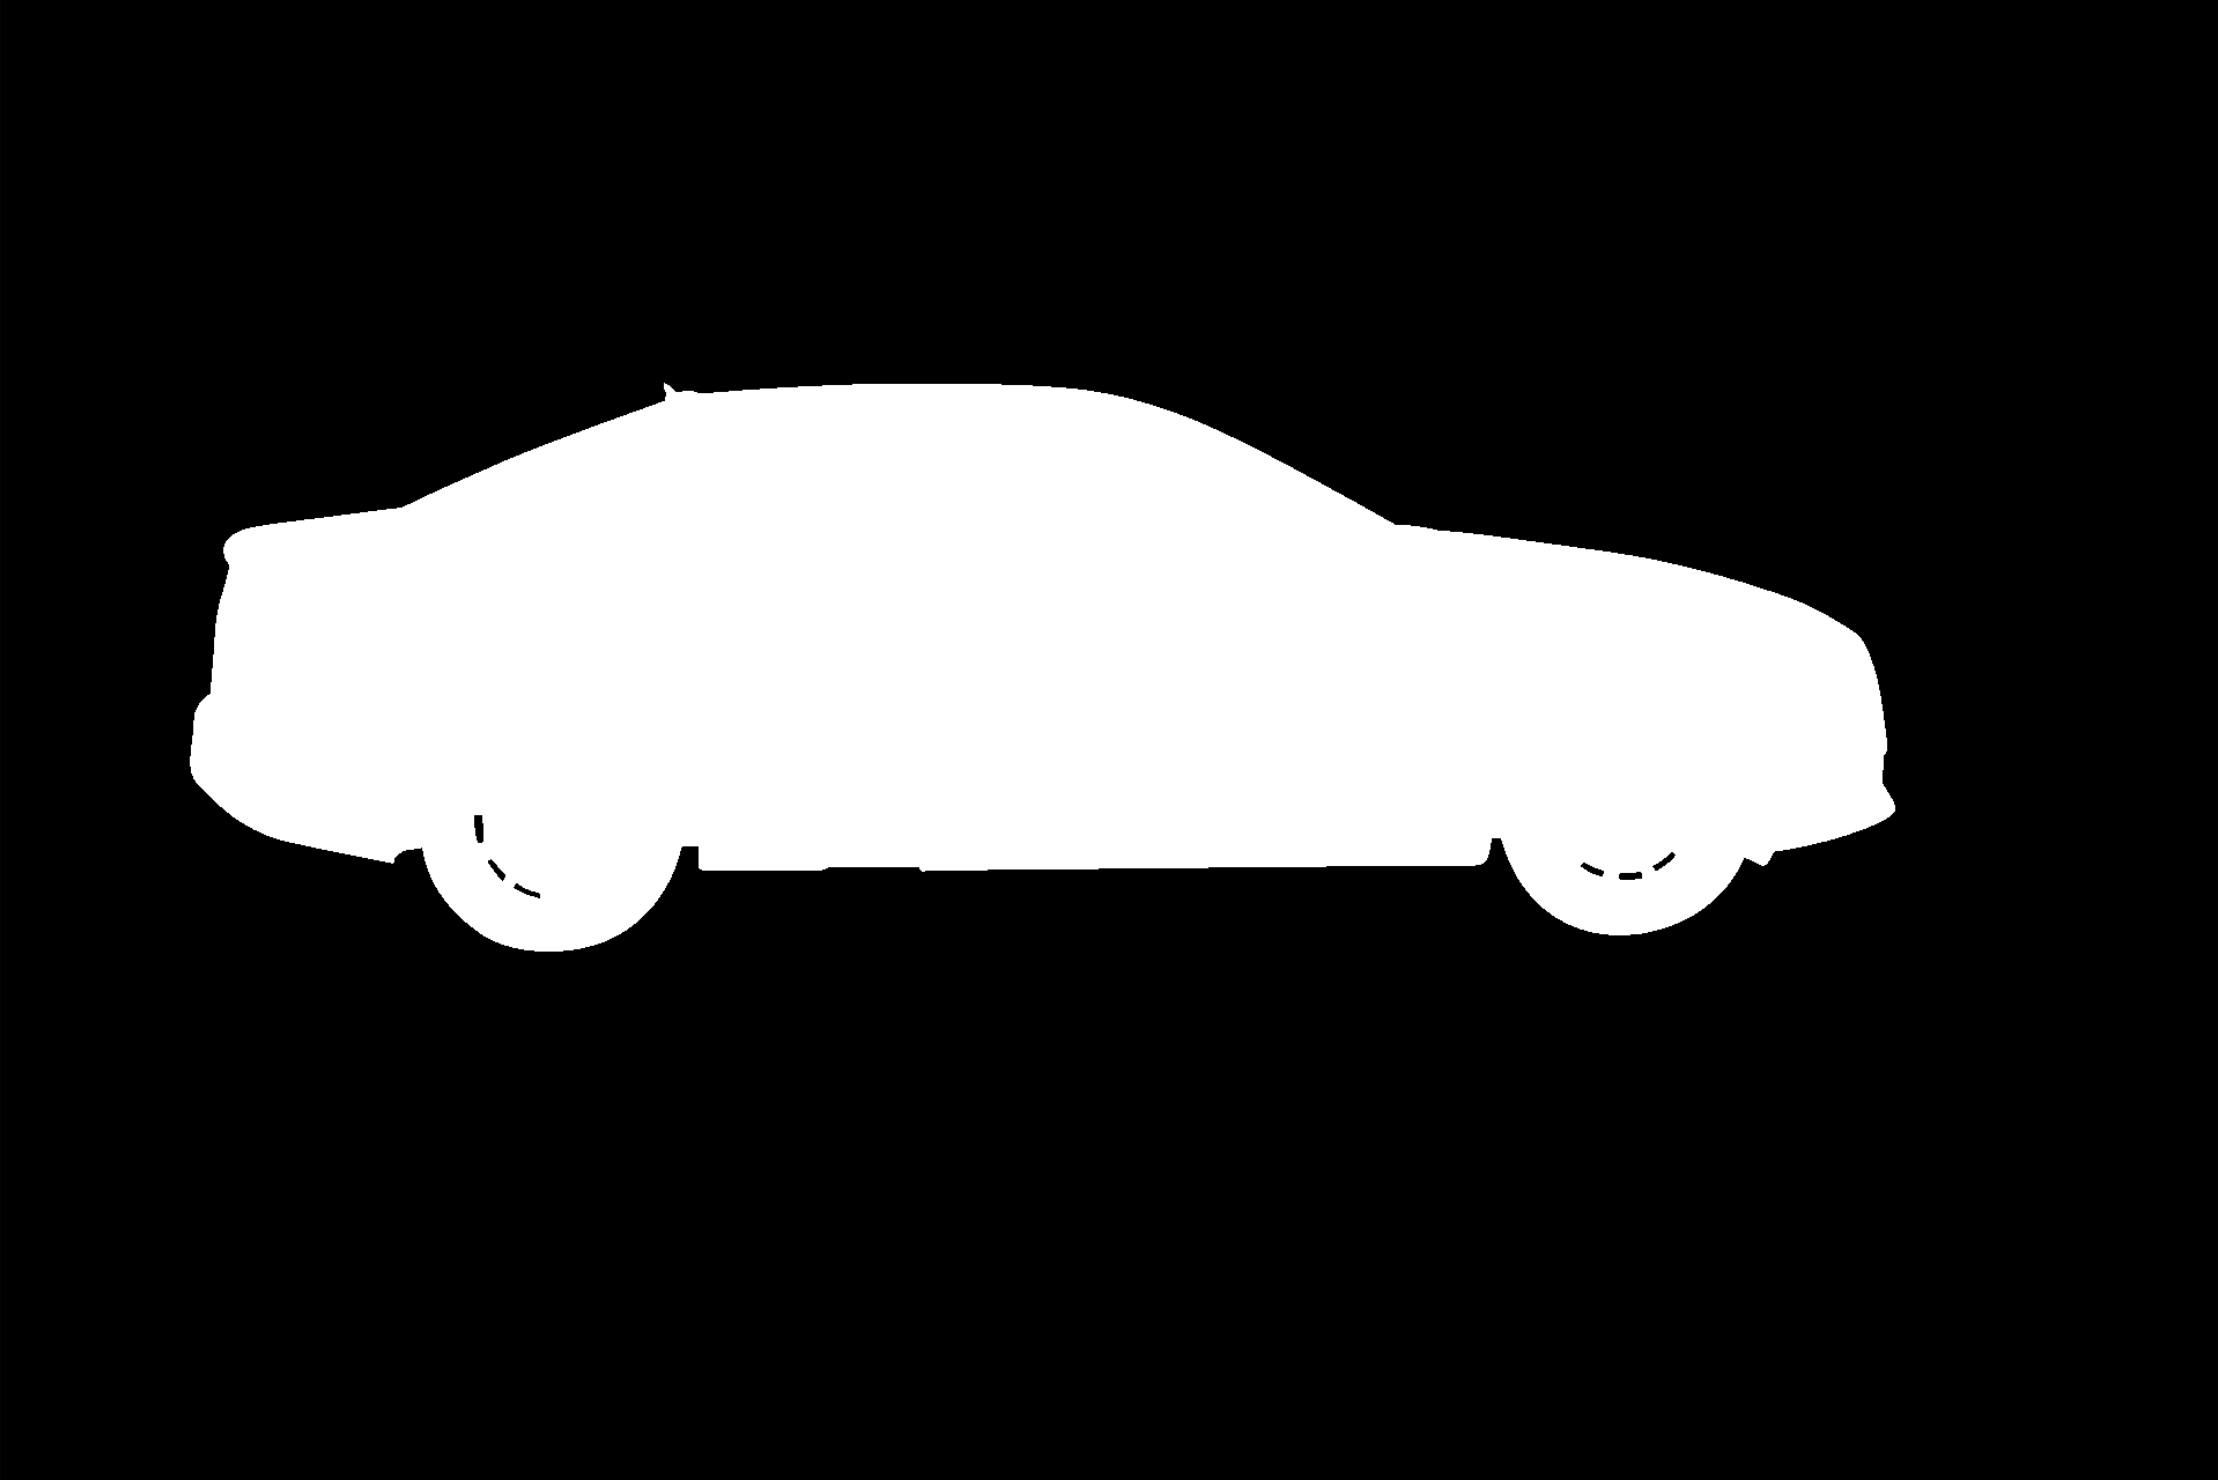
\includegraphics[width=4.5cm]{mask_true1.png}
            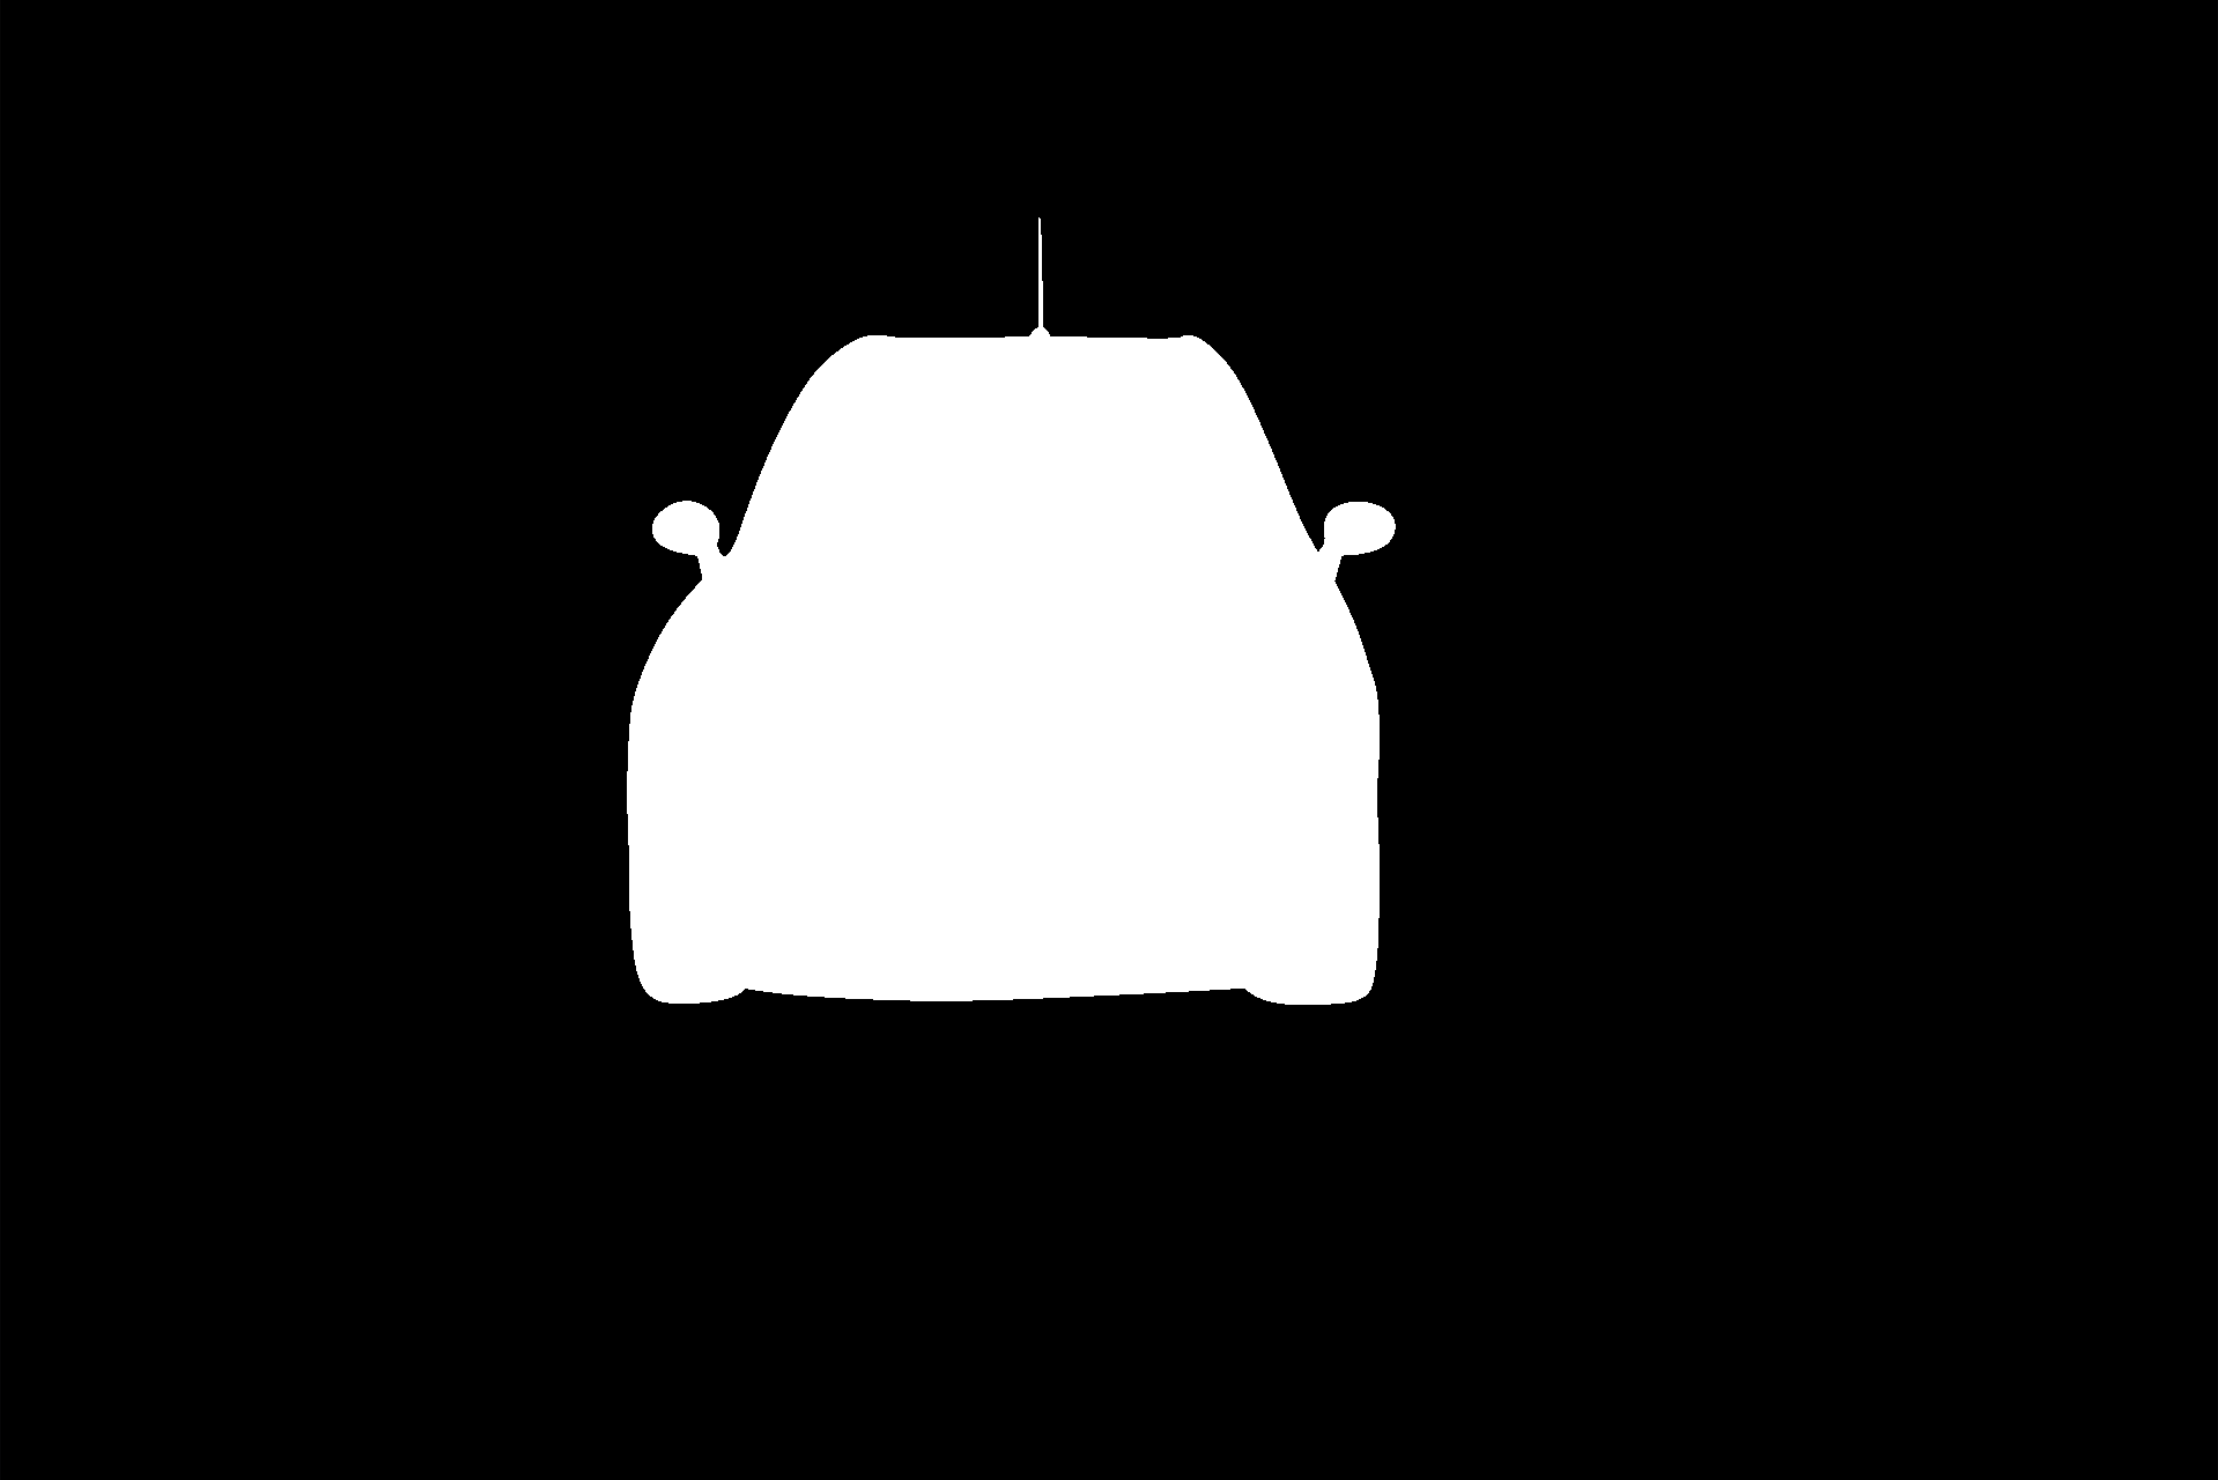
\includegraphics[width=4.5cm]{mask_true2.png}
            %\caption{fig2}
        \end{minipage}%
    }%
    \quad
    \subfloat[添加EdgeLoss项]{
        \begin{minipage}[t]{1.0\linewidth}
            \centering
            \includegraphics[width=4.5cm]{mask_edge.jpg}
            \includegraphics[width=4.5cm]{mask_edge1.jpg}
            \includegraphics[width=4.5cm]{mask_edge2.jpg}
            %\caption{fig2}
        \end{minipage}
    }%
    \quad
    \subfloat[不添加EdgeLoss项]{
        \begin{minipage}[t]{1.0\linewidth}
            \centering
            \includegraphics[width=4.5cm]{mask_noedge.jpg}
            \includegraphics[width=4.5cm]{mask_noedge1.jpg}
            \includegraphics[width=4.5cm]{mask_noedge2.jpg}
            %\caption{fig2}
        \end{minipage}
    }%
    \centering
    \caption{分割图对比}
    \label{mask_compare}
\end{figure}


















\begin{figure}[htbp]
    \centering
    \begin{minipage}[t]{0.45\linewidth}  %并排插图时,线宽很重要,自己慢慢试,俩张图就不要超过0.5,三张图不要超过0.33之类的,自己看着办  
        \centering
        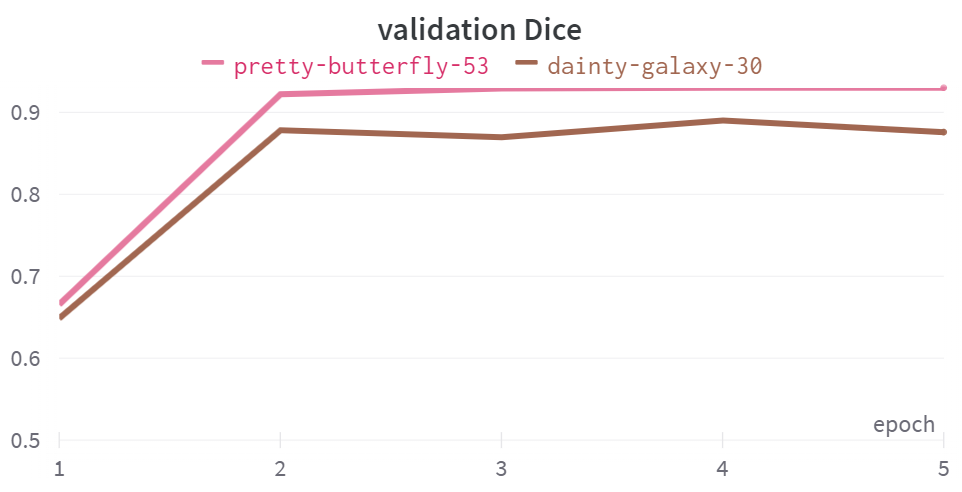
\includegraphics[height=4cm]{model_dice_no_aug.png}
        \caption{不进行数据增强操作,改进U-net对照结果}
        \label{model_dice_no_aug}
    \end{minipage}
    \hfill%分栏的意思吧
    \begin{minipage}[t]{0.45\linewidth}
        \centering
        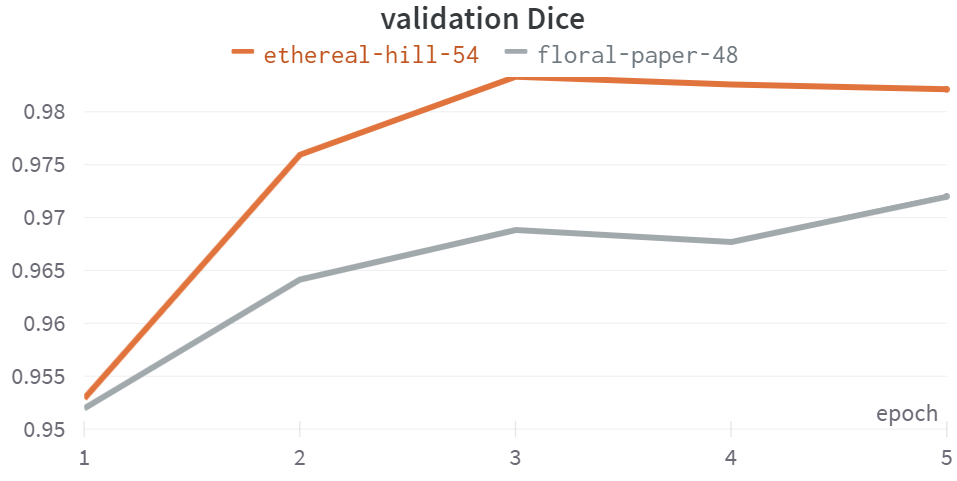
\includegraphics[height=4cm]{model_dice_aug.png}
        \caption{进行数据增强操作,改进U-net对照结果}
        \label{model_dice_aug}
    \end{minipage}
    % \caption{mask图和edge图}
\end{figure}



\begin{table}[htbp] %表格位置
    \setlength{\abovecaptionskip}{0cm}
    \setlength{\belowcaptionskip}{0.2cm}
    \centering
    \caption{分析对比实验设计}
    \label{aug_result}
    \begin{tabular}{|c|c|c|c|}
        \hline
        \diagbox{运行名称}{abc} & 数据增强 & EdgeLoss损失项 & 模型      \\
        \hline
        dainty-galaxy-30        & 否       & 不添加         & U-net     \\
        \hline
        drawn-pine-44           & 否       & 添加           & U-net     \\
        \hline
        floral-paper-48         & 是       & 不添加         & U-net     \\
        \hline
        crimson-morning-49      & 是       & 添加           & U-net     \\
        \hline
        preety-butterfly-53     & 否       & 不添加         & 改进U-net \\
        \hline
        ethereal-hill-54        & 是       & 不添加         & 改进U-net \\
        \hline
        dulcet-sun-56           & 否       & 添加           & 改进U-net \\
        \hline
        fresh-glade-55          & 是       & 添加           & 改进U-net \\
        \hline
    \end{tabular}
\end{table}



\begin{equation}
    \begin{aligned}
         & 3\times3\mbox{卷积核进行特征提取和通道融合:}64 \times 3 \times 3 \times 3=1728 \hfill                                           \\
         & 3\times 3\mbox{卷积核特征提取}+ 1\times 1\mbox{通道融合:}3 \times 1 \times 3 \times 3+ 64 \times 3 \times 1 \times 1=219 \hfill \\
         & 3\times3\mbox{卷积核进行特征提取和通道融合:}64\times 3\times1 \times 1  =192 \hfill                                             \\
         & \frac{1728-(219+192)}{219}\approx 6.01\hfill \nonumber
    \end{aligned}
\end{equation}
\begin{equation}
    \begin{split}
        3\times3\mbox{卷积核进行特征提取和通道融合:}64 \times 3 \times 3 \times 3=1728 \hfill \\
        3\times 3\mbox{卷积核特征提取}+ 1\times 1\mbox{通道融合:}3 \times 1 \times 3 \times 3+ 64 \times 3 \times 1 \times 1=219 \hfill \\
        3\times3\mbox{卷积核进行特征提取和通道融合:}64\times 3\times1 \times 1  =192 \hfill \\
        \frac{1728-(219+192)}{219}\approx 6.01\hfill \nonumber
    \end{split}
\end{equation}

\begin{equation}
    \begin{aligned}
         &  & 3\times3\mbox{卷积核进行特征提取和通道融合:}64 \times 3 \times 3 \times 3=1728                                           & \\
         &  & 3\times 3\mbox{卷积核特征提取}+ 1\times 1\mbox{通道融合:}3 \times 1 \times 3 \times 3+ 64 \times 3 \times 1 \times 1=219 & \\
         &  & 3\times3\mbox{卷积核进行特征提取和通道融合:}64\times 3\times1 \times 1  =192                                             & \\
         &  & \frac{1728-(219+192)}{219}\approx 6.01\nonumber                                                                           &
    \end{aligned}
\end{equation}


这是一个引用\textsuperscript{\cite{zhang2017mixup,RN08}}
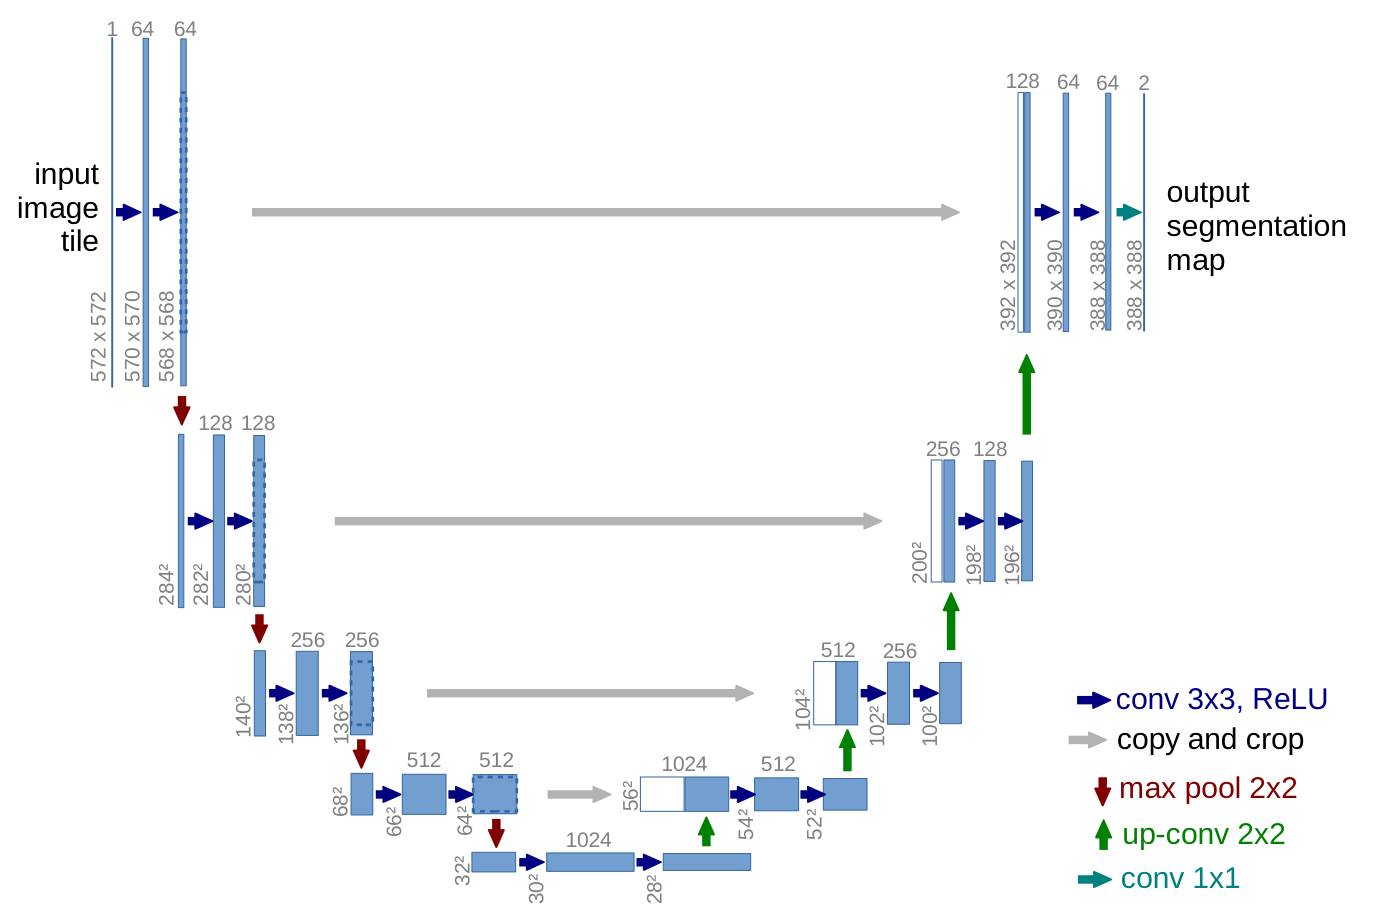
\includegraphics[scale=0.6]{u-net.png}
% \textsc{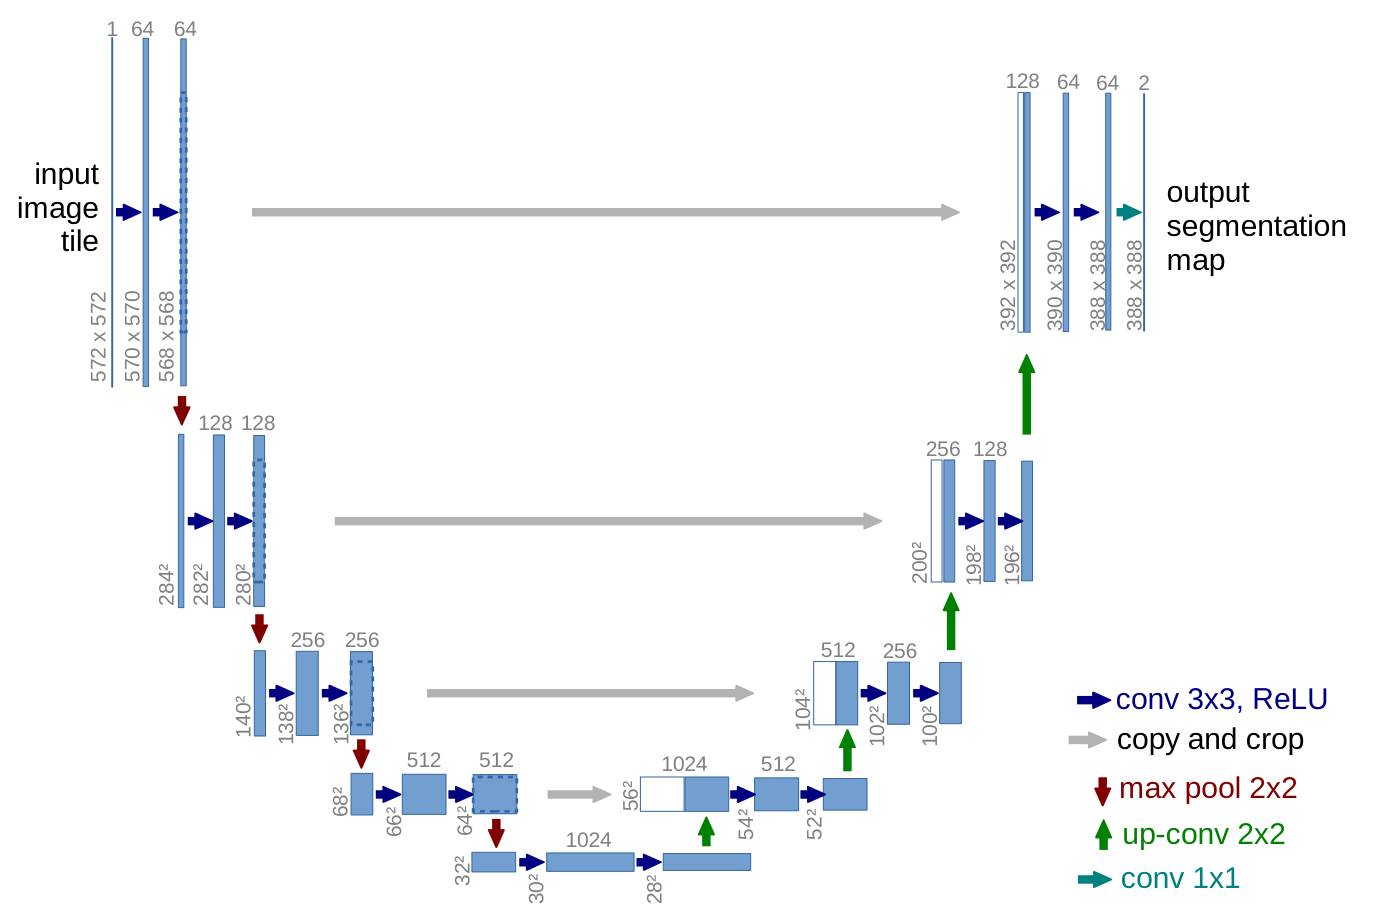
\includegraphics[height=0.5\textheight]{u-net.png}}
% 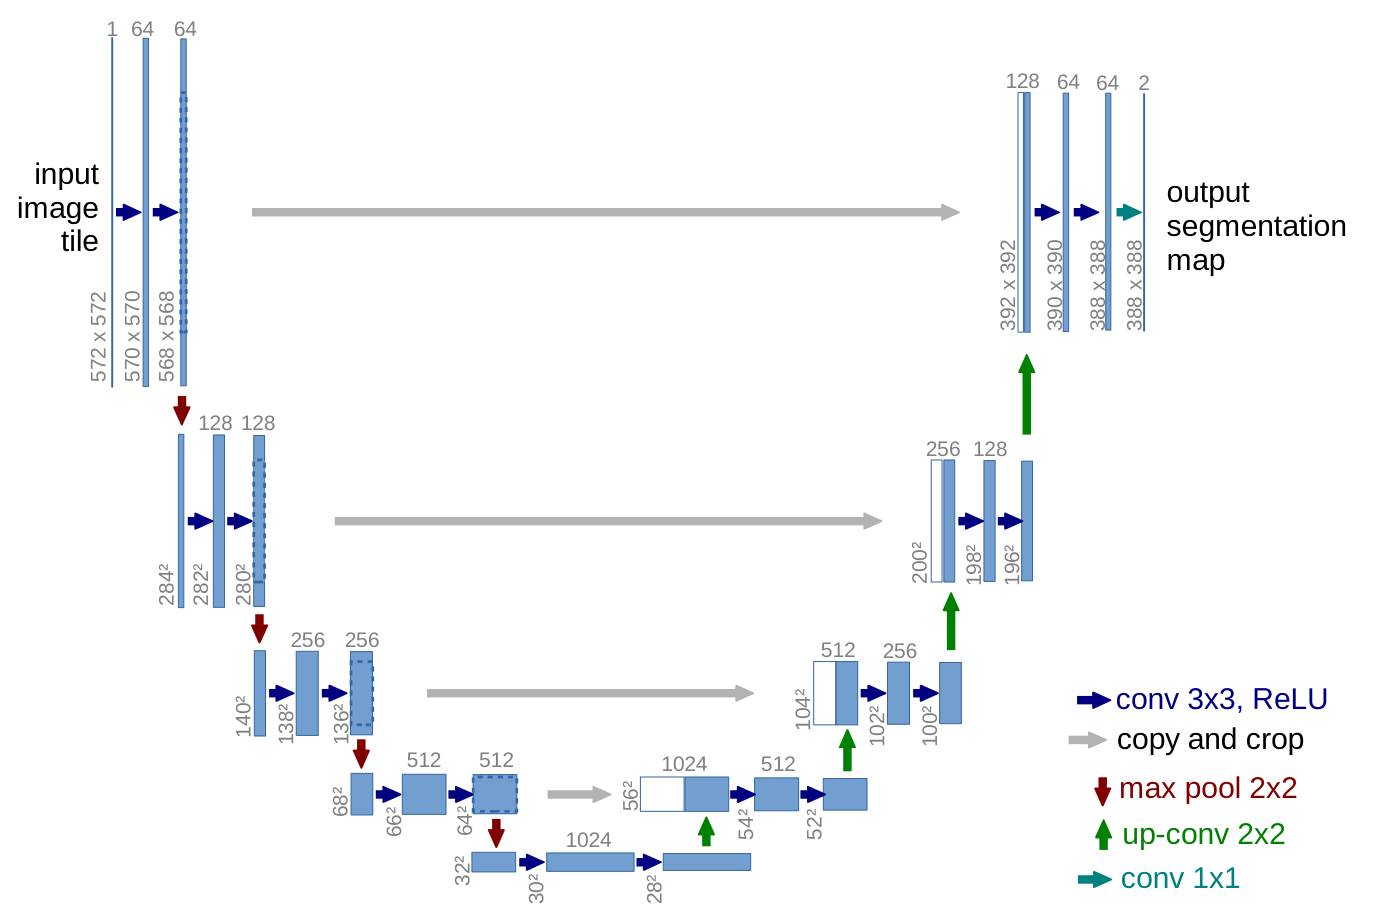
\includegraphics[width=0.2\textwidth]{u-net.png}
\begin{figure}[htbp]
    \begin{minipage}[t]{0.5\linewidth}  %并排插图时,线宽很重要,自己慢慢试,俩张图就不要超过0.5,三张图不要超过0.33之类的,自己看着办  
        \centering
        \includegraphics[height=4cm]{original_invert.jpg}
        \label{fig4}
        \caption{原始图像}
    \end{minipage}
    \hfill%分栏的意思吧
    \begin{minipage}[t]{0.5\linewidth}
        \centering
        \includegraphics[height=4cm]{invert_image.jpg}
        \label{fig5}
        \caption{invert操作图像}
    \end{minipage}
\end{figure}



\begin{figure}[htbp]
    \centering
    \begin{minipage}[t]{0.4\linewidth}  %并排插图时,线宽很重要,自己慢慢试,俩张图就不要超过0.5,三张图不要超过0.33之类的,自己看着办  
        \centering
        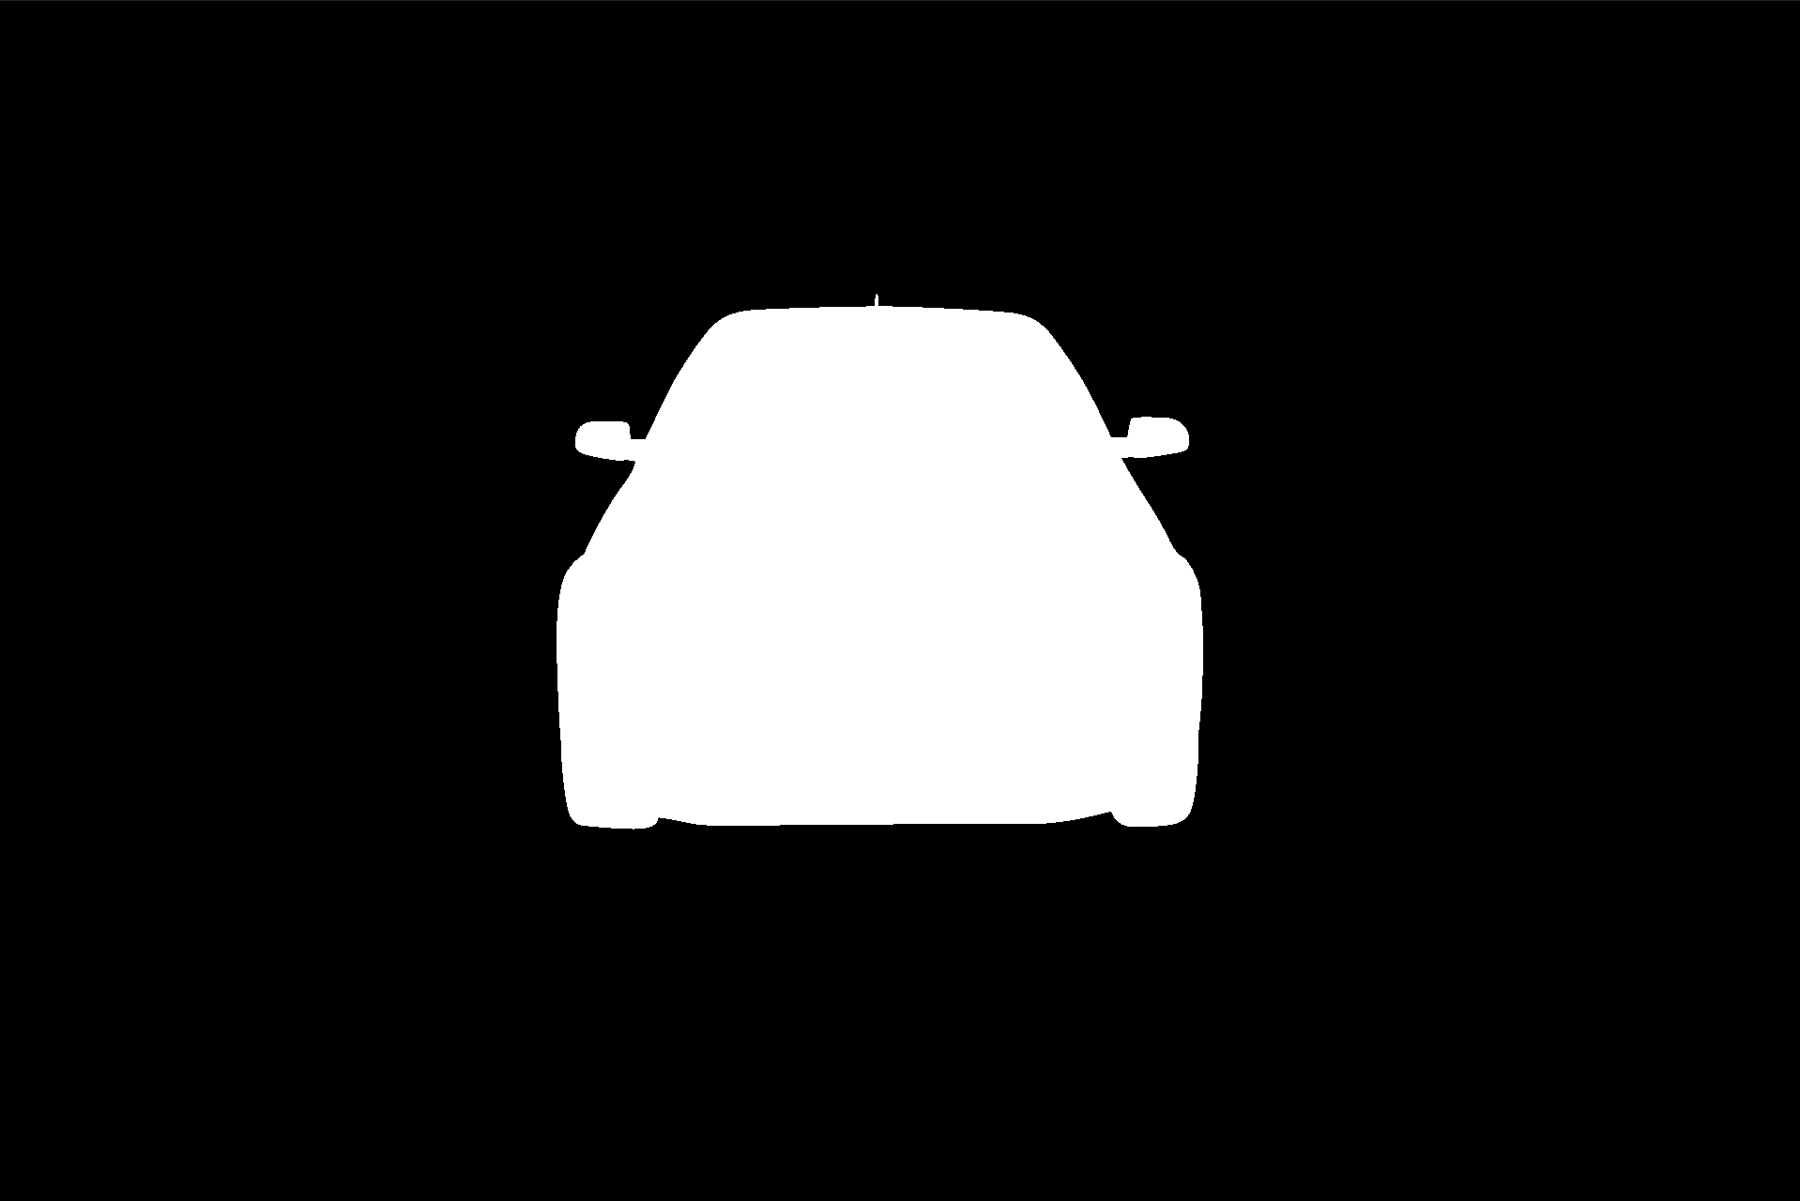
\includegraphics[height=5cm]{mask.png}
        % \caption{mask}
    \end{minipage}
    \hfill%分栏的意思吧
    \begin{minipage}[t]{0.5\linewidth}
        \centering
        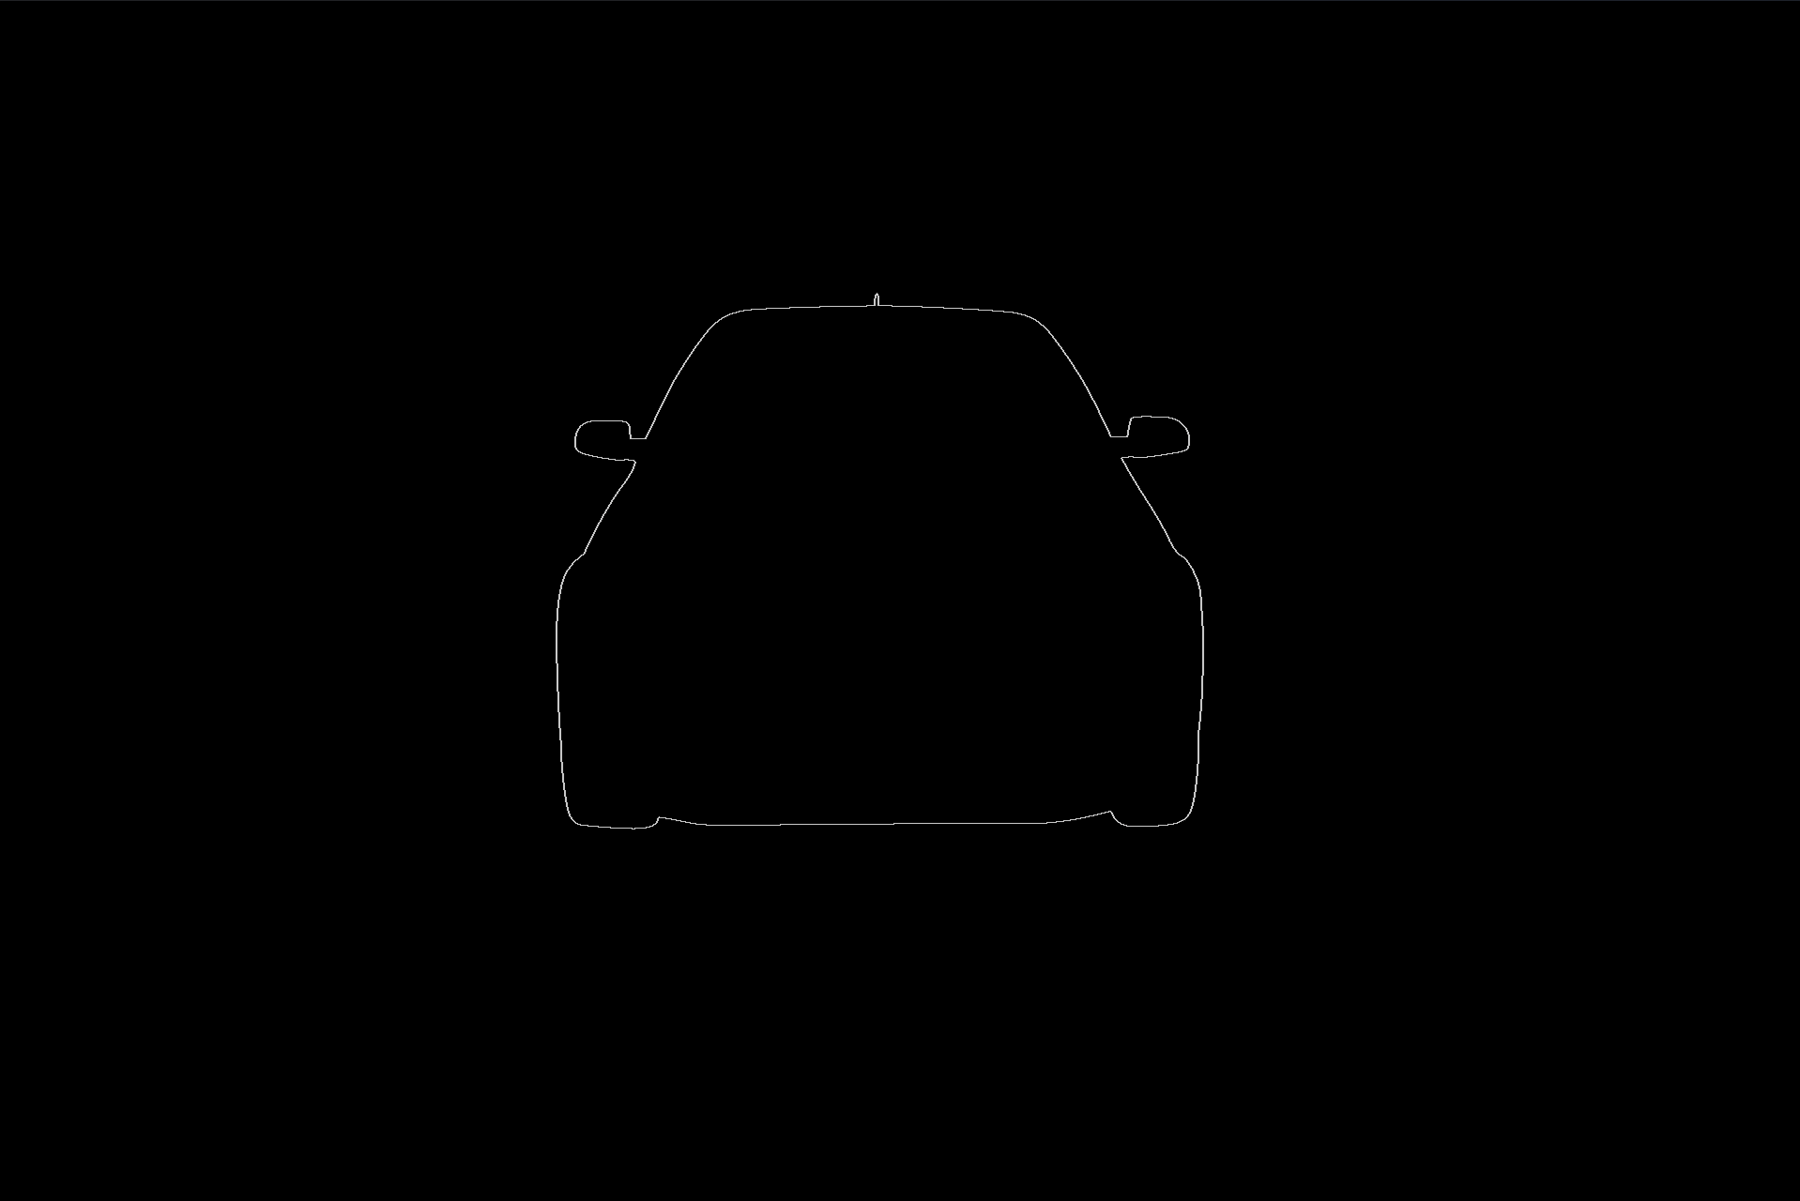
\includegraphics[height=5cm]{edge_outline.png}
        % \caption{edge}
    \end{minipage}
    \caption{mask图和edge图}
\end{figure}





\begin{figure}[htbp]
    \centering
    \subfloat[原始图像]{
        \begin{minipage}[t]{0.5\linewidth}
            \centering
            \includegraphics[width=6cm]{mask_image.jpg}
            %\caption{fig1}
        \end{minipage}%
    }%
    \subfloat[真实分割图]{
        \begin{minipage}[t]{0.5\linewidth}
            \centering
            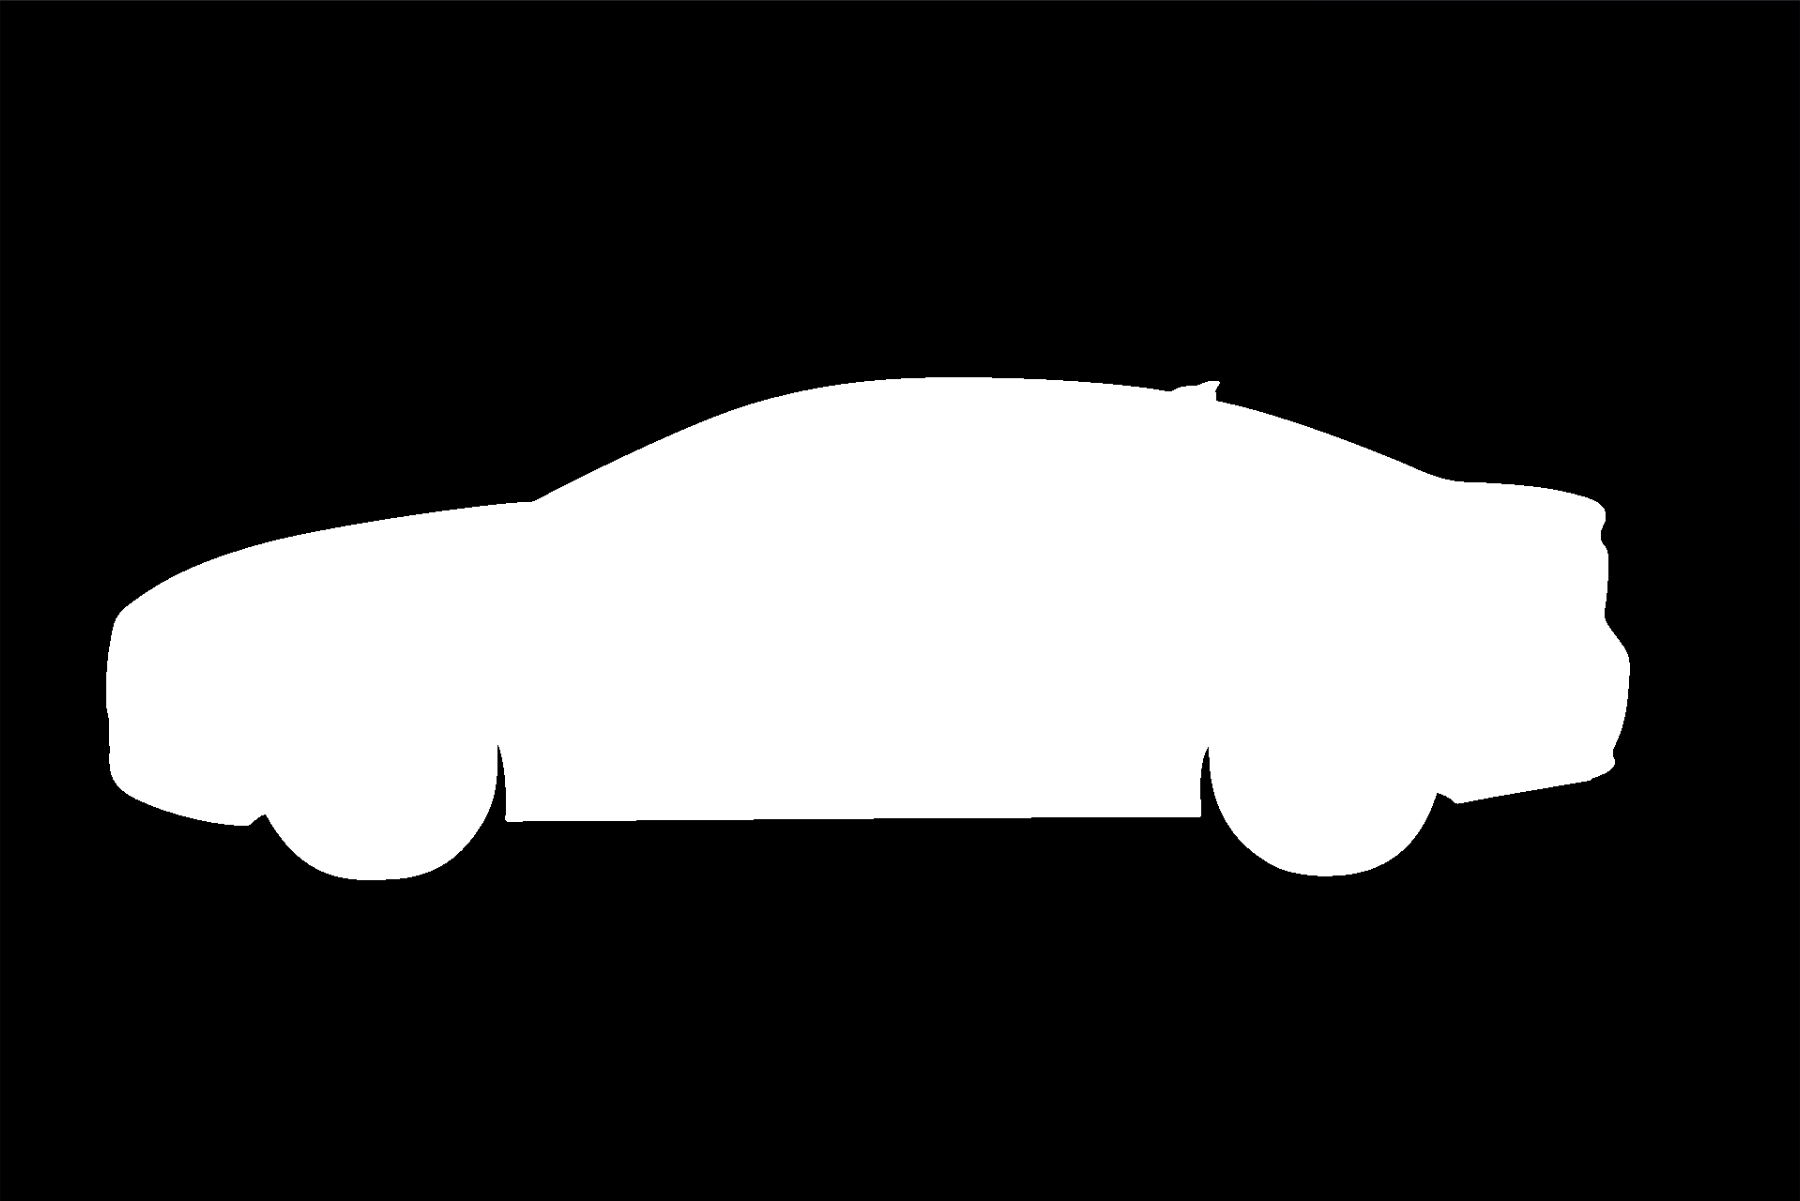
\includegraphics[width=6cm]{mask_true.png}
            %\caption{fig2}
        \end{minipage}%
    }%
    \quad
    \subfloat[添加EdgeLoss项]{
        \begin{minipage}[t]{0.5\linewidth}
            \centering
            \includegraphics[width=6cm]{mask_edge.jpg}
            %\caption{fig2}
        \end{minipage}
    }%
    \subfloat[不添加EdgeLoss项]{
        \begin{minipage}[t]{0.5\linewidth}
            \centering
            \includegraphics[width=6cm]{mask_noedge.jpg}
            %\caption{fig2}
        \end{minipage}
    }%
    \centering
    \caption{分割图对比}
    \label{mask_compare}
\end{figure}

\begin{tabular}{|c|c|c|}
    \hline
    数据增强操作             & 训练次数(epoch) & Dice相似系数 \\
    \hline
    不进行数据增强操作       & 5               & 0.8902       \\
    \hline
    不进行数据增强操作       & 10              & 0.9019       \\
    \hline
    invert                   & 5               & 0.5905       \\
    \hline
    hflip                    & 5               & 0.9311       \\
    \hline
    rotate                   & 5               & 0.9288       \\
    \hline
    affineScale              & 5               & 0.9301       \\
    \hline
    translateX               & 5               & 0.8976       \\
    \hline
    GaussianBlur             & 5               & 0.9036       \\
    \hline
    ColorJitter\_hue0.5      & 5               & 0.9231       \\
    \hline
    ColorJitter\_contrast0.5 & 5               & 0            \\
\end{tabular}


\begin{table}[htbp] %表格位置
    \setlength{\abovecaptionskip}{0cm}
    \setlength{\belowcaptionskip}{0.2cm}
    \centering
    \caption{数据增强操作}
    \label{tab:l1}
    \begin{tabular}{|c|c|c|}
        \hline
        数据增强操作             & 训练次数(epoch) & Dice相似系数 \\
        \hline
        不进行数据增强操作       & 5               & 0.8902       \\
        \hline
        不进行数据增强操作       & 10              & 0.9019       \\
        \hline
        invert                   & 5               & 0.5905       \\
        \hline
        hflip                    & 5               & 0.9311       \\
        \hline
        rotate                   & 5               & 0.9288       \\
        \hline
        affineScale              & 5               & 0.9301       \\
        \hline
        translateX               & 5               & 0.8976       \\
        \hline
        GaussianBlur             & 5               & 0.9036       \\
        \hline
        ColorJitter\_hue0.5      & 5               & 0.9231       \\
        \hline
        ColorJitter\_contrast0.5 & 5               & 0            \\
        \hline
    \end{tabular}
\end{table}
\bibdatabase{bib/database}%bib文件名称 仅修改bib/ 后部分
\printbib
\end{document}